% THIS IS SIGPROC-SP.TEX - VERSION 3.1
% WORKS WITH V3.2SP OF ACM_PROC_ARTICLE-SP.CLS
% APRIL 2009
%
% It is an example file showing how to use the 'acm_proc_article-sp.cls' V3.2SP
% LaTeX2e document class file for Conference Proceedings submissions.
% ----------------------------------------------------------------------------------------------------------------
% This .tex file (and associated .cls V3.2SP) *DOES NOT* produce:
%       1) The Permission Statement
%       2) The Conference (location) Info information
%       3) The Copyright Line with ACM data
%       4) Page numbering
% ---------------------------------------------------------------------------------------------------------------
% It is an example which *does* use the .bib file (from which the .bbl file
% is produced).
% REMEMBER HOWEVER: After having produced the .bbl file,
% and prior to final submission,
% you need to 'insert'  your .bbl file into your source .tex file so as to provide
% ONE 'self-contained' source file.
%
% Questions regarding SIGS should be sent to
% Adrienne Griscti ---> griscti@acm.org
%
% Questions/suggestions regarding the guidelines, .tex and .cls files, etc. to
% Gerald Murray ---> murray@hq.acm.org
%
% For tracking purposes - this is V3.1SP - APRIL 2009

\documentclass{acm_proc_article-sp}

\makeatletter
\let\@copyrightspace\relax
\makeatother

% Schusterjunge und co.
 \clubpenalty = 5000
 \widowpenalty = 5000
 \displaywidowpenalty = 5000

\usepackage{balance}
\usepackage{url}
\usepackage{listings}
\usepackage{graphicx}
\usepackage{subcaption}
\usepackage{capt-of}
\captionsetup[subfigure]{labelformat = parens, labelsep = space, font = small}
\usepackage[noend]{algpseudocode}
\usepackage{color}
\usepackage{pgfplots}
\usepackage{filecontents}
\usepackage{epstopdf}

\begin{document}
\title{Code Generation in ExaHyPE}%Interim Evaluation}
\subtitle{Handover Document}
%\subtitle{\small{... as part of the `Seminar on Advanced and Mobile Internet Technology'}\\
%\small{\mbox{https://www.comsys.rwth-aachen.de/teaching/ws-1415/seminars-on-advanced-and-mobile-internet-technology/}}
%}
%\titlenote{A full version of this paper is available as
%\textit{Author's Guide to Preparing ACM SIG Proceedings Using
%\LaTeX$2_\epsilon$\ and BibTeX} at
%\texttt{www.acm.org/eaddress.htm}}}
%
% You need the command \numberofauthors to handle the 'placement
% and alignment' of the authors beneath the title.
%
% For aesthetic reasons, we recommend 'three authors at a time'
% i.e. three 'name/affiliation blocks' be placed beneath the title.
%
% NOTE: You are NOT restricted in how many 'rows' of
% "name/affiliations" may appear. We just ask that you restrict
% the number of 'columns' to three.
%
% Because of the available 'opening page real-estate'
% we ask you to refrain from putting more than six authors
% (two rows with three columns) beneath the article title.
% More than six makes the first-page appear very cluttered indeed.
%
% Use the \alignauthor commands to handle the names
% and affiliations for an 'aesthetic maximum' of six authors.
% Add names, affiliations, addresses for
% the seventh etc. author(s) as the argument for the
% \additionalauthors command.
% These 'additional authors' will be output/set for you
% without further effort on your part as the last section in
% the body of your article BEFORE References or any Appendices.

\numberofauthors{1} %  in this sample file, there are a *total*
% of EIGHT authors. SIX appear on the 'first-page' (for formatting
% reasons) and the remaining two appear in the \additionalauthors section.
%
\author{
% You can go ahead and credit any number of authors here,
% e.g. one 'row of three' or two rows (consisting of one row of three
% and a second row of one, two or three).
%
% The command \alignauthor (no curly braces needed) should
% precede each author name, affiliation/snail-mail address and
% e-mail address. Additionally, tag each line of
% affiliation/address with \affaddr, and tag the
% e-mail address with \email.
%
% 1st. author
\alignauthor
AS, 8.9.2016
%Angelika Schwarz
      %\affaddr{}
      % \affaddr{1932 Wallamaloo Lane}\\
      % \email{angelika.schwarz@rwth-aachen.de}
}

\date{\today}
% Just remember to make sure that the TOTAL number of authors
% is the number that will appear on the first page PLUS the
% number that will appear in the \additionalauthors section.

\maketitle
\begin{abstract}
  Approaching the exascale era, scientific codes are forced to adapt in order to harness the computational resources. Research groups typically do not develop an application code completely on their own, but use well-optimised libraries as back end. ExaHyPE as a solver engine for hyperbolic PDEs addresses this need and  will provide scalable and efficient kernels for large-scale computer systems. A key step towards a high-performance code is achieving good single-core performance. Hardware-aware programming, smart memory layouts and vectorisation provide the means to it. For this purpose, ExaHyPE employs a code generator, which couples driver routines with back end assembly code generation. This report documents the current status of the code generator and present first performance results.
\end{abstract}

% A category with the (minimum) three required fields
%\category{H.4}{Information Systems Applications}{Miscellaneous ???}
%A category including the fourth, optional field follows...
%\category{D.2.8}{Software Engineering}{Metrics}[complexity measures, performance measures ???]

%\terms{Theory}

%\keywords{???} % NOT required for Proceedings

% structure:
%  \section
%  \subsection
%  \subsubsection
%

\section{Introduction} \label{sec1}
The ExaHyPE project develops an engine that utilises the high-order discontinuous Galerkin (DG) finite element method \cite{dumbser2014posteriori,dumbser2015high} in order to solve hyperbolic PDEs. It provides a foundation to simulate astrophysics or geoscience scenarios at exascale level. ExaHyPE comprises the following basic building blocks.

\begin{itemize}
\item \textbf{Toolkit}. The toolkit acts as the user interface. It reads in a specification file, selects solver kernels and outputs glue code. The specification file contains parameters such as the computational domain, the order of the DG polynomial, and optimisation options. %If the parameters are set in a particular way, the toolkit triggers the code generation described below.
\item \textbf{Adaptive Mesh Management}. The adaptive Cartesian grid is implemented by the Peano framework \cite{Software:Peano}.
\item \textbf{Solver Kernels}. As part of an engine, there is a stock of generic, non-optimised compute kernels. A suited subset is selected and combined through the glue code of the toolkit. This subset is selected in accordance with the specification file. In particular, the subset depends on the type of problem (linear/non-linear PDE) specified by the user.
\item \textbf{Code Generator}. The code generator outputs optimised solver kernels for one particular specification file. For this set-up, the code generator decides on the memory layout, computation schemes, makefile options and prefetching strategies. 
\end{itemize}

ExaHyPE has to provide efficient solver kernels in order to utilise the computational resources of large-scale computer systems. The code generator of the ExaHyPE engine provides a means to replace the generic, non-optimised solver kernels with optimised ones. The code generator is therefore the key ingredient for achieving good single-core performance. 


Section~\ref{sec:math} introduces the ADER discontinuous Galerkin (DG) method as the numerical scheme. Section~\ref{sec:3} discusses the current status of the code generator and presents first performance results. 

\section{ADER DG Scheme}\label{sec:math}
The ExaHyPE engine addresses hyperbolic conservation laws in 2 or 3 space dimensions. In the remainder of this report, the focus in on nonlinear hyperbolic conservation laws of the form
\begin{align}\frac{\partial \mathbf{Q}}{\partial t} + \nabla \cdot \mathbf{F}(\mathbf{Q}) = 0, \qquad \mathbf{x}\in \Omega, t \in \mathbb{R}_{\geq 0}\label{eq:pde}\end{align}
subject to an initial condition $\mathbf{Q}(\mathbf{x},0)$, where $\mathbf{x}\in \Omega$, and boundary conditions $\mathbf{Q}(\mathbf{x},t) = \mathbf{Q}_{Bnd}(\mathbf{x},t)$, where $\mathbf{x}\in \partial \Omega$. Here $\mathbf{Q}\in \mathbb{R}^{V}$ denotes the $V$-valued vector of conserved quantities, $\mathbf{F}(\mathbf{Q})$ a non-linear flux tensor, and $\Omega$ the two-dimensional and three-dimensional computational domain, respectively. 

Following \cite{dumbser2014posteriori,dumbser2015high}, ExaHyPE employs a Cartesian grid to discretise the computational domain
\begin{align*}
\Omega = \dot{\bigcup \limits_k} T^k.
\end{align*}
The elements $T^k$ are cubes in 3D or squares in 2D. ExaHyPE uses nodal DG to represent the solution approximation in each element through a polynomial of degree $N$
\begin{align*}\mathbf{u}_h^k(\mathbf{x}, t^n) = \sum \limits_{i=0}^{N} \Phi_i(\mathbf{x}) \hat{\mathbf{u}}_i^n, \mathbf{x} \in T^k.\end{align*}
The basis functions $\Phi_i(\mathbf{x})$ are given by the tensor product of the Lagrange interpolation polynomials evaluated at the Gauss-Legendre nodes; $\hat{\mathbf{u}}_i^n$ denotes the degrees of freedom at time $t^n$. The direct sum of the element-wise DG polynomials gives the global discrete solution. 

ExaHyPE employs a predictor-corrector scheme to evolve the solution. First, the predictor computes an element-local space-time DG solution $\mathbf{q}_h$. Second, the corrector incorporates influences from neighbouring cells into the element-local solution $\mathbf{q}_h$ and updates thereby the true DG solution $\mathbf{u}_h$.

For a unified numerical scheme, the elements $T^k$ are mapped onto a space-time reference element. The spatial coordinates in the reference elements are $\mathbf{\xi} = (\xi, \eta)$ in 2D and $\mathbf{\xi} = (\xi, \eta, \zeta)$ in 3D, respectively; the temporal variable is $t = t^n + \tau \Delta t$. Given $d$ space dimensions, $T_E = [0,1]^d$ describes the space reference element and $T_E\times[0,1]$ the space-time reference element. In the reference element, the PDE reads as
\begin{align}
\frac{\partial \mathbf{Q}}{\partial \tau} + \nabla_{\xi}\cdot \mathbf{F}^*(\mathbf{Q}) = 0 \label{eq:pdereference}
\end{align}
where $\nabla_{\mathbf{\xi}} = \partial \mathbf{\mathbf{\xi}}/\partial \mathbf{x} \cdot \nabla$ is the gradient with respect to the reference coordinates and $\mathbf{F}^*(\mathbf{Q}) = \Delta t(\partial \mathbf{\xi}/\partial \mathbf{x})^T \cdot \mathbf{F}(\mathbf{Q})$ is the volume flux in the reference element.

Multiplying the PDE in Equation~(\ref{eq:pdereference}) with space-time test functions \mbox{$\Theta_k = \Theta_k(\mathbf{\xi}, \tau)$} and integrating over the space-time reference element yields the weak form
\begin{align}
\int \limits_{0}^{1} \int \limits_{T_E} \Theta_k \frac{\partial \mathbf{Q}}{\partial \tau} d\mathbf{\xi} d \tau+ \int \limits_{0}^{1} \int \limits_{T_E} \Theta_k \nabla_\xi \cdot \mathbf{F}^*_h(\mathbf{Q}) d\mathbf{\xi} d\tau = 0.\label{eq:weakformreference}
\end{align}

\subsection{Space-time Predictor}\label{sec2:1}
The space-time predictor computes a local solution in the space-time reference element. Given some space-time test functions $\Theta(\mathbf{\xi}, \tau)$, the predictor solution in reference coordinates is
\begin{align}
\mathbf{q}_h(\mathbf{\xi},\tau) = \sum \limits_{l=0}^{N} \Theta_l(\mathbf{\xi}, \tau) \hat{\mathbf{q}}_l \label{eq:qh}
\end{align}
and the space-time volume flux  is
\begin{align}
\mathbf{F}^*_h(\mathbf{\xi},\tau) = \sum \limits_{l=0}^{N} \Theta_l(\mathbf{\xi}, \tau) \hat{\mathbf{F}}^*_l. \label{eq:fh}
\end{align}
The latter amounts to the evaluation of the flux function at the Gauss-Legendre nodes, i.e. $\hat{\mathbf{F}}_l^* = \mathbf{F}^*(\hat{\mathbf{q}}_l)$. Inserting the predictor solution $\mathbf{q}_h$ into Equation~(\ref{eq:weakformreference}) yields
\begin{align*}
\int \limits_{0}^{1} \int \limits_{T_E} \Theta_k \frac{\partial \mathbf{q}_h}{\partial \tau} d\mathbf{\xi} d \tau+ \int \limits_{0}^{1} \int \limits_{T_E} \Theta_k \nabla_\xi \cdot \mathbf{F}^*_h d\mathbf{\xi} d\tau = 0.
\end{align*}
Integrating the first term by parts in time results in
\begin{align*}
\left[ \int \limits_{T_E} \Theta_k \frac{\partial \mathbf{q}_h}{\partial \tau} d\mathbf{\xi} \right]^1_0 &- \int \limits_{0}^{1} \int \limits_{T_E} \frac{\partial \Theta_k}{\partial \tau}\mathbf{q}_h d\mathbf{\xi}d\tau  \\
&+ \int \limits_{0}^{1} \int \limits_{T_E} \Theta_k \nabla_\xi \cdot \mathbf{F}^*_h d\mathbf{\xi} d\tau = 0.
\end{align*}
The first term is now in the form to connect the predictor solution and the DG solution. At the beginning of each time step, the DG solution serves as the initial condition for the space-time predictor:
\begin{align*}
\left[ \int \limits_{T_E} \Theta_k \frac{\partial \mathbf{q}_h}{\partial \tau} d\mathbf{\xi} \right]^1 &- \left[ \int \limits_{T_E} \Theta_k \frac{\partial \mathbf{u}_h}{\partial \tau} d\mathbf{\xi} \right]^0 - \int \limits_{0}^{1} \int \limits_{T_E} \frac{\partial \Theta_k}{\partial \tau}\mathbf{q}_h d\mathbf{\xi}d\tau  \\
&+ \int \limits_{0}^{1} \int \limits_{T_E} \Theta_k \nabla_\xi \cdot \mathbf{F}^*_h d\mathbf{\xi} d\tau = 0.
\end{align*}
Inserting Equation~(\ref{eq:qh}) and Equation~(\ref{eq:fh}) leads to the space-time predictor solver kernel used in ExaHyPE:

\begin{align}
\begin{split}
&\sum \limits_{l=0}^N \underbrace{\left( \int \limits_{T_E} \Theta_k(\xi,1) \Theta_l(\xi,1) d\xi - \int \limits_{0}^{1} \int \limits_{T_E} \frac{\partial \Theta_k}{\partial \tau} \Theta_l d\xi d\tau \right)}_{\mathbf{K}_1} \hat{\mathbf{q}}_l = \\
&\underbrace{\sum \limits_{l=0}^N \left( \int \limits_{T_E} \Theta_k(\xi,0) \Phi_l d\xi\right) \hat{\mathbf{u}}_l^n}_{\text{\textbf{rhs0}}} \\
&\qquad - \sum \limits_{l=0}^N \underbrace{\left( \int \limits_{0}^1 \int \limits_{T_E} \Theta_k \nabla_{\mathbf{\xi}}  \Theta_l d\mathbf{\xi} d\tau \right)}_{\nabla_{\mathbf{\xi}} \mathbf{K}_{\xi}} \mathbf{F}^*(\hat{\mathbf{q}}_l)\label{eq:final}
\end{split}
\end{align}
The space-time predictor is the computationally most expensive component in the ADER-DG scheme. It is split up into three solver kernels.
\begin{itemize}
\item \textbf{Picard Loop.} Based on Equation~(\ref{eq:final}), Picard iterations\footnote{In the linear case, the Picard loop is replaced by the Cauchy-Kowalewski time evolution.} approximate the space-time predictor coefficients $\hat{\mathbf{q}}_l$. As $\mathbf{K}_1$ is entirely based on the reference element, its inverse is precomputed.
\begin{align*}
  \mathbf{K}_1 \hat{\mathbf{q}}^{r+1}_l &= \text{\textbf{rhs0}} - \nabla_{\mathbf{\xi}} \mathbf{K}_\xi \mathbf{F}^*(\hat{\mathbf{q}}_l^r) \\
  \Rightarrow \qquad \hat{\mathbf{q}}^{r+1}_l &= \mathbf{K}_1^{-1} (\text{\textbf{rhs0}} - \nabla_{\mathbf{\xi}} \mathbf{K}_\xi \mathbf{F}^*(\hat{\mathbf{q}}_l^r))
\end{align*}
After $r=N$ iterations, the space-time evolved predictor coefficients are known.

\item \textbf{Time Averaging.} Time-averaging of the volume flux and the predictor over $[t^n, t^{n+1}]$ concludes the time integration.
\begin{align}\label{eq:timeaveraging}
\begin{split}
\bar{\mathbf{F}}^* = \sum \limits_{l} w_l \hat{\mathbf{F}}^*_l\\
\bar{\mathbf{q}} = \sum \limits_{l} w_l \hat{\mathbf{q}}_l
\end{split}
\end{align}

\item \textbf{Boundary Extrapolation.} As ExaHyPE uses nodal DG evaluated at the Gauss-Legendre nodes, the predictor and the flux values attained at the boundaries must still be computed. For this purpose, the values are extrapolation to the left and to the right end of the reference element 
\begin{align*}
\bar{\mathbf{q}}^- &= \sum \limits_l \Phi_l(0) \bar{\mathbf{q}}_l\\
\bar{\mathbf{q}}^+ &= \sum \limits_l \Phi_l(1) \bar{\mathbf{q}}_l.
\end{align*}
The flux is extrapolated analogously.
\end{itemize}
The predictor solution is local to an element and does not consider fluxes from neighbouring elements. The corrector stage augments the predictor solution by such contributions and thereby advances the DG solution to the next time step.

\subsection{Corrector}\label{sec2:2}

The weak form of the PDE in Equation~(\ref{eq:pde}) is obtained by 
multiplying with a spatial test function $\Phi_i(\mathbf{x})$, integrating over the space-time control volume \mbox{$T^k \times [t^n, t^{n+1}]$}, and reducing smoothness requirements on the flux function through integrating the flux divergence term
\begin{align*}
\int \limits_{t^n}^{t^{n+1}} \int \limits_{T^k} \Phi_i \frac{\partial \mathbf{Q}}{\partial t} d\textbf{x}dt &+  \int \limits_{t^n}^{t^{n+1}} \int \limits_{\partial T^k} \Phi_i \mathbf{F}(\mathbf{Q})\cdot \mathbf{n} \, dS dt \\ &- \int \limits_{t^n}^{t^{n+1}} \int \limits_{T^k}\nabla \Phi_i \cdot \mathbf{F}(\mathbf{Q}) \, d\mathbf{x}dt = 0
\end{align*}
where $\partial T^k$ denotes the boundary of the element $T^k$ and $\mathbf{n}$ its outward-pointing unit normal vector.

Inserting the predictor polynomial $\mathbf{q}_h$ given in Equation~(\ref{eq:qh}) yields the discretised form. The boundary flux term amounts to a Riemann problem given the time-averaged boundary data $\bar{\mathbf{q}}^-$, $\bar{\mathbf{q}}^+$, extrapolated from the left and the right element onto the face. As such, it is replaced with a numerical flux function in normal direction $\mathcal{G}(\bar{\mathbf{q}}^-,\bar{\mathbf{q}}^+)\cdot \mathbf{n}$. Altogether, the ADER-DG scheme reads
\begin{align}\label{eq:corrector2}
\begin{split}
\sum \limits_l \underbrace{\left(\int \limits_{T^k} \Phi_i \Phi_l d\mathbf{x} \right)}_{\mathbf{M}} &\left(\hat{\mathbf{u}}_l^{n+1} - \hat{\mathbf{u}}_l^{n} \right) \\
&+ \underbrace{\int \limits_{t^n}^{t^{n+1}} \int \limits_{\partial T^k} \Theta_i \mathcal{G}(\bar{\mathbf{q}}^-,\bar{\mathbf{q}}^+)\cdot \mathbf{n} \, dS dt}_{\Delta \bar{\mathbf{f}}} \\
&- \underbrace{\int \limits_{t^n}^{t^{n+1}} \int \limits_{T^k} \nabla \Phi_k \cdot \mathbf{F}(\mathbf{q}_h) \, d\mathbf{x} dt}_{\mathbf{K}_\xi \bar{\mathbf{F}}^*} = 0.
\end{split}
\end{align} 
As the mass matrix $\mathbf{M}$ is diagonal and assembles the tensor product of $N$ Gauss-Legendre weights $\mathbf{w}$, the explicit scheme becomes
\begin{align}
\begin{split}
\label{eq:predictorscheme}
\mathbf{M}\Delta \hat{\mathbf{u}} &= \mathbf{K}_\xi \bar{\mathbf{F}}^* - \Delta \bar{\mathbf{f}} \\
\Rightarrow \qquad \hat{\mathbf{u}}^{n+1} &=  \hat{\mathbf{u}}^n + \frac{\Delta t}{\mathbf{w}} \left(\mathbf{K}_\xi \bar{\mathbf{F}}^* - \Delta \bar{\mathbf{f}} \right).
\end{split}
\end{align}

The corrector comprises two solver kernels.
\begin{itemize}
\item \textbf{Volume Kernel.} The volume integral computes the correction term $\mathbf{K}_\xi \bar{\mathbf{F}}^*$ and is the computationally secondmost expensive component.
\item \textbf{Boundary Kernel.} The surface integral including the Riemann solver constitutes the boundary kernel, which computes the term $\Delta \bar{\mathbf{f}}$. For this purpose, ExaHyPE utilises a Rusanov solver.
\end{itemize}
Eventually the incorporation of the weighted correction term concludes one time step.

\section{Project Status}\label{sec:3}
ExaHyPE's code generator aims at replacing the generic solver kernels with vectorised, optimised version. For this purpose, the following questions have been tackled.
\begin{itemize}
\item What is the structure of the matrices and tensors?
\item What is the favourable memory layout for each kernel? How can conflicting memory layouts be resolved?
\item What is the access pattern to the tensors?
\item What is the best way to multiply the square system matrix with a tensor slice?
\item What parts of the code can be handled by an auto-vectorising compiler?
\end{itemize}
 
Due to usage of Cartesian grids, the solver kernels rely on dense, small-sized tensor operations. The most prominent operation is the matrix-tensor multiply. In this setup, the matrix resembles a square system matrix such as $\mathbf{K}_{\mathbf{\xi}}$. The tensor comprises degrees of freedom of the quantities in one element. In a 2D domain, for example, the tensor constitutes a three-way tensor holding the degrees of freedom for the quantities in $x$- and in $y$-direction.


\paragraph{Structure}\label{paragraph:structure}
The system matrices are small, the tensors are tall and thin. In the nonlinear case all structures are dense. There is no sparsity pattern that could be taken into account for the computations. Due to the small size of the matrices, they can be assumed to reside in the cache.

\paragraph{Memory Layout}\label{paragraph:memorylayout}
The tensors store the degrees of freedom of all quantities in each spatial direction, possibly also in time. For a 2D setup, a spatial tensor is a three-way tensors with the dimensions (i) the quantities $Q$, (ii) the degrees of freedom in $x$-direction $DOFx$, and (iii) the degrees of freedom in $y$-direction $DOFy$. The dimensions of the tensor can be reordered freely, which yields a smattering of different ordering schemes. The solver kernels indeed favour certain ordering schemes. The space-time predictor exhibits weighted matrix-tensor multiplies. Since the weights apply to the quantities, the preferred ordering is $(Q,DOFx,DOFy)$. For the boundary kernel, by contrast, the data should be ordered as $(DOFx,Q_{Bnd})$ and $(DOFy, Q_{Bnd})$. The volume integral works on dimension-dependent flux tensors, which can be split and ordered independently. Figure~\ref{fig:code} illustrates this. In summary, the individual solver kernels favour conflicting ordering schemes. A switch between ordering schemes typically requires that the tensor is transposed.


\paragraph{Access Pattern}\label{paragraph:accesspattern}
Closely related to the different ordering schemes of the tensor dimensions is the access pattern to the tensors. For a 2D setup, the simplest occurrence of a weighted matrix-tensor multiply is
$$\mathbf{C}(:,:,j) = \alpha(j) \mathbf{B}(:,:,j) \mathbf{A}(:,:)$$ followed with $$\mathbf{C}(:,i,:) = \alpha(i) \mathbf{B}(:,i,:)\mathbf{A}(:,:).$$ 
This operation is prominent in the space-time predictor. The scalar $\alpha$ is a quadrature weight. The matrix $\mathbf{A}(:,:)$ is a fixed square system matrix. The tensor $\mathbf{B}(:,:,:)$ stores the degrees of freedom for all quantities. Here, its first dimension holds the quantities; its other two dimensions hold the spatial degrees of freedom in the $x$- and the $y$- direction, respectively. Due to the Cartesian grid set-up, the directions (here $x$- and $y$-direction) are processed one after another and demand different slices $\mathbf{B}(:,:,j)$ and $\mathbf{B}(:,i,:)$ of the tensor. As a result, the way the tensors are accessed depends on the  spatial direction.
\paragraph{Multiplication Order}\label{paragraph:multiplicationorder}
There are two orders in which matrices can be multiplied, namely $\mathbf{A}\mathbf{B}$ vs $\mathbf{B}^T \mathbf{A}^T$. For ExaHyPE, this affects the choice of the memory layout. Section~\ref{sec:libxsmmPerformanceStudy} takes up on this topic. 

\subsection{Code Generator}\label{sec3:1}
Due to the access patterns to the tensors, the optimised kernels process the matrix-tensor multiplies in the form of a sequence of small-sized strided matrix-matrix multiplies. For this purpose, the code generator holds sequences of configurations. Consider for example a matrix-vector multiply. A configuration then specifies the dimensions of the matrix and the one of the vector. Based on these configurations, the code generator outputs two types of files.
\begin{itemize}
\item \textbf{Implementation files.} The code generator holds sequences of configurations. Each configuration yields an implementation file. Such an implementation file is typically given in the form of assembly code or close-to-assembly code. The latter can be intrinsics code or simple-structured C code that can be processed by an auto-vectorising compiler.
\item \textbf{Driver files.} Driver files wrap the calls to the implementation files. The tensor set-up performs the very same operation on one data structure, but with different start addresses. A large part of code generator is therefore dedicated to the computation of the start addresses for the given configurations. %As such, a driver routine implements a sequence of configurations. 
\end{itemize}
The combination of driver routines and implementation files will substitute the generic solver kernels. ExaHyPE's code generator utilises Intel's libxsmm as assembly code generation back end. Most of the implementation files are generated with Intel's libxsmm. Given a sequence of slices of a tensor, the matrix-tensor multiply becomes a sequence of dense weighted matrix-matrix multiplications. %As Intel's libxsmm does not support arbitrary scalars, the tensor product of the quadrature weights is incorporated into the system matrix before the gemm call.




\subsection{Optimisation of Selected Kernels}



\paragraph{Picard Loop}
Based on the DG solution of the previous time step, the Picard loop computes the space-time evolved coefficients $\hat{\mathbf{q}}$ of the predictor polynomial. In the latest version of ExaHyPE, only the generic C++ kernels are in use; the generic Fortran kernels are only a legacy version. While the generic C++ kernels process matrix-tensor multiplies in an element-by-element fashion, the generic Fortran kernels use built-in intrinsics. The optimised version implements the Picard loop as follows.
\begin{algorithmic}
\State $\text{\textbf{rhs0}} = \sum \limits_{l=0}^N\left( \int \limits_{T^k} \Theta_k(\xi,0) \Phi_l d\xi \right) \hat{\mathbf{u}}_l^n$
\For{$r = 0, \ldots, N$}
\State $\mathbf{K}_{\xi}^s = \nabla_{\xi} \mathbf{K}_{\xi} $
\State $\text{\textbf{rhs}} = \text{\textbf{rhs0}} - \mathbf{K}_{\xi}^s \mathbf{F}^*(\hat{\mathbf{q}}_l^r)$
\State $\hat{\mathbf{q}}^{r+1} = \text{\textbf{rhs}} \left(\mathbf{K}_1^{-1}\right)^T$
\EndFor
\end{algorithmic}

As Intel's libxsmm does not support arbitrary scalars, the $d$-dimensional discrete scalar product over the reference element is incorporated into the auxiliary matrix $K_\xi^s$. 
The right-hand side is accumulated through a sequence of gemm calls. ExaHyPE stores all matrices and tensor slices in column major format. In contrast to Equation~\ref{eq:predictorscheme}, \textbf{rhs0} and \textbf{rhs} therefore are implicitly transposed so that $(\mathbf{K}_1^{-1})^T$ is multiplied from the right. Internally, the optimised version holds both $\mathbf{K}_1^{-1}$ and its transpose  $(\mathbf{K}_1^{-1})^T$ in memory to avoid any transpose operations.   %In contrast to Equation~\ref{eq:predictorscheme}, rhs0 and rhs store transposed tensors slices so that $\mathbf{K}_1^{-1}$ is multiplied from the right. 

The optimised version excels at order 7 because the dimension of the tensor slices exactly equals the SIMD width. Order 8, by contrast, falls off. For compatibility with the generic kernels, only some data structures have been padded; in particular the data structure holding the frequently used \textbf{rhs} remains unpadded.

The coupling of the optimimised kernels and the user-defined flux function imposes an unfavourable memory layout for the flux tensor. ExaHyPE will provide fully optimised examples with an optimised data layout of the flux tensor and an vectorised evaluation of the flux function. 

Anticipating Section~\ref{sec:libxsmmPerformanceStudy}, changing the multiplication order from $\mathbf{K}_{\xi}^s \mathbf{F}^*(\hat{\mathbf{q}}_l^r)$ to $\mathbf{F}^*(\hat{\mathbf{q}}_l^r) \mathbf{K}_{\xi}^s$ in conjunction with batched BLAS promises further speedup. Moreover, alignment of the data structures is yet to be done.

\paragraph{Volume Kernel}
The volume kernel computes the contribution of the volume integral as given in Equation~\ref{eq:corrector2} to the update tensor $\Delta \hat{\mathbf{u}}^n$. The optimised version implements the volume integral as follows.

\begin{algorithmic}
  \State $\mathbf{K}_{\xi}^s = \frac{\mathbf{w}}{\Delta x_\xi} \mathbf{K}_{\xi}^T$
\State $\Delta \hat{\mathbf{u}}^n = \bar{\mathbf{F}}^* \mathbf{K}_{\xi}^s$
\end{algorithmic}

Following Paragraph~\ref{paragraph:accesspattern}, the spatial directions are processed successively.
Due to the assumption of isotropic elements, the volume kernel works independent of the spatial direction being accessed. Following the workaround proposed by \cite{libxsmmconversation}, the $d$-dimensional discrete scalar product over the reference element is incorporated into the auxiliary matrix $\mathbf{K}_{\xi}^s$ and used repeatedly. The spatial contributions are therefore interleaved rather than processed one after another.

While all system matrices and the tensor slices $\bar{\mathbf{F}}^*$ are padded, the update tensor $\Delta \hat{\mathbf{u}}^n$ is not. The transition from order 7 to order 8 suggests that the introduction of padding for  the update tensor gives further speedup. Moreover, all tensors are unaligned.

The manual version of the optimised kernels demonstrates the feasibility of the batched BLAS idea, see Section~\ref{sec:libxsmmPerformanceStudy}. This version is hand-written assembly code where 6 matrix-matrix multiplies are computed jointly. The hand-written code covers only the $x$-direction. The runtime reported is only an extrapolated value, assuming that processing each direction takes equally long. Possible memory effects are therefore not included.


\paragraph{Time Averaging}
The time-integrated fluxes and predictor coefficients are obtained by averaging the space-time evolved quantities. The optimised kernels interpret Equation~(\ref{eq:timeaveraging}) as a sequence of matrix-matrix multiplies of a $Q$-by-$N$ with an $N$-by-1 matrix, which is handed over to Intel's libxsmm. 


\subsection{Performance of Selected Kernels} 
This section compares the generic kernels (Fortran and C++) and the optimised version, compiled on Intel C++ compiler (\texttt{icpc version 15.0.4}) with \texttt{-O2 -xHost} and Intel Fortran compiler (\texttt{ifort version 15.0.4}) with \texttt{-O2 -r8 -align -fpp -xHost}. 

All measurements have been executed on an Intel Xeon E5-2690v3 (``Haswell'') operating at 2.6 GHz and Intel Xeon Phi 7250 (``Knights Landing (KNL)'') at 1.40GHz. One Haswell core processes 2 Fused Multiply Add (FMA3) vector instructions per cycle and exhibits 256-bit wide AVX instructions so that 4 double-precision operands can be processed simultaneously. Its peak performance calculates as 2.6 Ghz $\cdot 2 \cdot 2 \cdot 4 = 41.6$ GFlops/s \footnote{\url{https://www.lrz.de/services/compute/supermuc/systemdescription/}}. One KNL core processes 2 FMA3 per cycle with 512-bit wide AVX-512 instructions instead and operates at 1.4GHz, its peak performance calculates as 1.4 $\cdot 2 \cdot 2 \cdot 8 = $ 44.8GFlops/s. The test case covers the 3D Euler equations of fluid dynamics with five, nine, twenty-three and fifty-six variables for the polynomial degrees 3 up to 8.

{\color{red}Overall measurements with more quantities showed better performances for the optimized kernels as showed in appendix \ref{sec:app1}. KNL measurements showed more instabilities as the ones done on Haswell as showed in appendix \ref{sec:app2}.}

% peak performance
\begin{table*}
  \centering
\begin{tabular}{l|rrrrrr}
  \textbf{Order}                & \multicolumn{1}{c}{3}& \multicolumn{1}{c}{4}&\multicolumn{1}{c}{5}&\multicolumn{1}{c}{6}&\multicolumn{1}{c}{7}& \multicolumn{1}{c}{8}\\ \hline
\textbf{Picard loop}            &&&&&&\\
 ~~~~- flop count                            & 135168& 543750 & 1586304& 3932838 & 8650752 & 18068994 \\ 
~~\textit{Haswell}            &&&&&&\\
 ~~~~- runtime [$\mu{}$s]               & 27.43  & 140.2   & 330.5   & 951.6    & 1530    & 3840  \\
 ~~~~- performance [Gflops/s]           & 4.92  & 3.88   & 4.80   & 4.13    & 5.65    & 4.71  \\
 ~~~~- efficiency [\%]                  & 11.8  & 9.3   & 11.5   & 9.9    & 13.6    & 11.3  \\ 
~~\textit{KNL}            &&&&&&\\
 ~~~~- runtime [$\mu{}$s]               & 71.22  & 270.1   & 528.3   & 2232    & 4060    & 9259  \\
 ~~~~- performance [Gflops/s]           & 1.90  & 2.01   & 3.00   & 1.76    & 2.13    & 1.95  \\
 ~~~~- efficiency [\%]                  & 4.26 & 4.50 & 6.72 & 3.94 & 4.77 & 4.37  \\ \hline
\textbf{Volume Kernel}                   & &&&&& \\
 ~~~~- flop count                            & 6976 & 17875  & 37368 & 69629 & 119296 & 194643 \\
~~\textit{Haswell}            &&&&&&\\
 ~~~~- runtime [$\mu$s]                 & 1.24  & 3.54   & 6.47   & 11.22    & 17.53   & 32.32  \\  
 ~~~~- performance [Gflops/s]           & 5.62  & 5.05   & 5.78   & 6.21    & 6.81    & 6.02  \\   
 ~~~~- efficiency [\%]                  & 13.5  & 12.1   & 13.9   & 14.9    & 16.3    & 14.5  \\
~~\textit{KNL}            &&&&&&\\ 
 ~~~~- runtime [$\mu$s]                 & 4.05  & 7.8   & 12.94   & 29.92    & 38.09    & 66.32  \\
 ~~~~- performance [Gflops/s]           & 1.72  & 2.29   & 2.89   & 2.32    & 3.13    & 2.93  \\ 
 ~~~~- efficiency [\%]                  & 3.85 & 5.13 & 6.47& 5.20 & 7.01 & 6.56  \\ \hline
\textbf{Time Averaging}                  &&&&& \\ 
 ~~~~- flop count                            & 8960 & 22500 & 47520 & 89180 & 153600 & 247860 \\
~~\textit{Haswell}            &&&&&&\\
 ~~~~- runtime [$\mu$s]                      & 2.02  & 5.15   & 10.19   & 19.92    & 34.85    & 53.11  \\
 ~~~~- performance [Gflops/s]                & 4.44  & 4.37   & 4.66   & 4.48    & 4.41    & 4.67  \\
 ~~~~- efficiency [\%]                       & 10.7  & 10.5   & 11.2   & 10.7    & 10.6    & 11.2  \\
~~\textit{KNL}            &&&&&&\\
 ~~~~- runtime [$\mu$s]                      & 7.29  & 14.55   & 29.38   & 54.31    & 142.47    & 231.42  \\
 ~~~~- performance [Gflops/s]                &  1.22 & 1.54   & 1.61   & 1.64   & 1.08    & 1.07  \\
 ~~~~- efficiency [\%]                       & 2.73 & 3.45 & 3.60 & 3.68 & 2.42 & 2.39  \\
\end{tabular}
% Example Picard N=3:   47952 = 4 [iters] * (74 [simd scale count] * (2 [\nabla_\xi] + 160 [libxsmm_flop_counter]))
%   #picard iters: 4
%   one call to gemm_5_4_4_rhs_x or gemm_5_4_4_rhs_y or gemm_5_4_4_rhs_z: 160 (2MNK)
%   number of calls to gemm_5_4_4_rhs_x or gemm_5_4_4_rhs_y or gemm_5_4_4_rhs_z: iters * 64
%   before each gemm call there is a scaling operation: 16*scaling (note that we do not count 2 multiplications but onlyl one)
%   total flops for processing x direction: 4 * 64 * (160 + 16)
%   total flops in picard loop (neglecting rhs0): 3 * [4 * 64 * (160 + 16)] = 135168 
%   
% Example Volume N=3:   7936  = 16 [nDOF**2] * ( 16 [simd scale] + 3 [3D] * 160 [libxsmm_flop_counter])
%   one simd call for each sweep over x,y,z: 16
%   processing one direction, i.e. gemm call, 2MN(2K-1) = 140
%   processing one weight: simd + 3* gemm call = 16 + 3*140
%   loop over dofs: nDOF**2 = 16
%   in total: 16 * (16 + 3 * 140) = 6976
\caption{Efficiency of the optimised kernels with respect to the theoretical peak performance of one core for 5 quantities on Haswell and KNL. The flop count for the Picard loop neglects the evaluation of the flux function and the computations of \textbf{rhs0}. The runtime of the Picard loop covers \textbf{rhs0}, but not the evaluation of the flux function. The manual version is hand-written assembly code which mimics batched BLAS. Only the $x$-direction with 6 jointly computed matrix-matrix multiplies has been implemented, the results reported here are extrapolated. }\label{tab:flopcount}
\end{table*}


\paragraph{Picard Loop}
Figures~\ref{fig:resultsPicard} shows the runtime measurements for the 3D case with 5 quantiites on Haswell.
For higher orders the optimised version yields a speedup of a factor of roughly 1.6 over the Fortran version which grows to 1.8 at 56 quantities. 

\begin{figure}
\begin{filecontents}{resultsPicard.dat}
% order fortran  optimised   generic
3,60,27,140
4,196,140,360
5,468,330,1030
6,1132,950,2540
7,2596,1530,5600
8,5556,3840,10810
% fluctuates heavily.
\end{filecontents}
\pgfplotsset{scaled y ticks=false}
\begin{tikzpicture}
\begin{axis}[xlabel={order},ylabel={Runtime in $\mu$s},legend style={at={(0,1)},anchor=north west}, legend cell align=left]
  
% Graph column 1 versus column 0
\addplot[color=red,mark=otimes*] table[x index=0,y index=1,col sep=comma] {resultsPicard.dat};
\addlegendentry{Generic Fortran} % columns left
 
% Graph column 2 versus column 0
\addplot[color=blue,mark=triangle*] table[x index=0,y index=2,col sep=comma] {resultsPicard.dat};
\addlegendentry{Optimised} % column middle

% Graph column 3 versus column 0
\addplot[color=black,mark=square*] table[x index=0,y index=3,col sep=comma] {resultsPicard.dat};
\addlegendentry{Generic C++} % column right

\end{axis}
\end{tikzpicture}
\caption{Haswell - Performance comparison of various implementations of the Picard loop without the evaluation of the 3D Euler flux function.}\label{fig:resultsPicard}
\end{figure}

% \begin{figure}
% \begin{filecontents}{resultsPicardKNL.dat}
% % order fortran  optimised   generic
% 3,346,71,1012
% 4,1181,270,3011
% 5,3495,528,7743
% 6,8402,2232,17228
% 7,18999,4060,34709
% 8,39906,9259,72608
% % fluctuates heavily.
% \end{filecontents}
% \pgfplotsset{scaled y ticks=false}
% \begin{tikzpicture}
% \begin{axis}[xlabel={order},ylabel={Runtime in $\mu$s},legend style={at={(0,1)},anchor=north west}, legend cell align=left]
  
% % Graph column 1 versus column 0
% \addplot[color=red,mark=otimes*] table[x index=0,y index=1,col sep=comma] {resultsPicardKNL.dat};
% \addlegendentry{Generic Fortran} % columns left
 
% % Graph column 2 versus column 0
% \addplot[color=blue,mark=triangle*] table[x index=0,y index=2,col sep=comma] {resultsPicardKNL.dat};
% \addlegendentry{Optimised} % column middle

% % Graph column 3 versus column 0
% \addplot[color=black,mark=square*] table[x index=0,y index=3,col sep=comma] {resultsPicardKNL.dat};
% \addlegendentry{Generic C++} % column right
% \end{axis}
% \end{tikzpicture}
% \caption{KNL - Performance comparison of various implementations of the Picard loop without the evaluation of the 3D Euler flux function.}\label{fig:resultsPicardKNL}
% \end{figure}

\paragraph{Volume Kernel}
Similar to the runtime measurements of the Picard loop, the optimised version is about a factor of 1.7 faster than the Fortran version, see Figure~\ref{fig:resultsVolume}. However the speedup grows to a factor 3.2 with 56 quantities as shown in appendix \ref{sec:app1}.

\begin{figure}
\begin{filecontents}{resultsVolume.dat}
3,3.17,1.24,3.99
4,6.62,3.54,9.7
5,12.86,6.47,19.25
6,21.56,11.22,34.63
7,35.27,17.53,57.93
8,54.06,32.32,91.47
\end{filecontents}
\begin{tikzpicture}
\begin{axis}[xlabel={order},ylabel={Runtime in $\mu$s},legend style={at={(0,1)},anchor=north west}, legend cell align=left]
  
% Graph column 2 versus column 0
\addplot[color=black,mark=square*] table[x index=0,y index=3,col sep=comma] {resultsVolume.dat};
\addlegendentry{Generic C++} % column right

% Graph column 3 versus column 0
\addplot[color=red,mark=otimes*] table[x index=0,y index=1,col sep=comma] {resultsVolume.dat};
\addlegendentry{Generic Fortran} % column left

% Graph column 1 versus column 0    
\addplot[color=blue,mark=triangle*] table[x index=0,y index=2,col sep=comma] {resultsVolume.dat};
\addlegendentry{Optimised} % column middle

\end{axis}
\end{tikzpicture}
\caption{Haswell - Performance comparison of the generic and optimised version of the volume kernel.}\label{fig:resultsVolume}
\end{figure}

% \begin{figure}
% \begin{filecontents}{resultsVolumeKNL.dat}
% 3,15.43,4.05,22.42
% 4,36.54,7.8,50.29
% 5,75.55,12.94,96.27
% 6,137.97,29.92,166.47
% 7,236.32,38.09,270.55
% 8,373.61,66.32,417.6
% \end{filecontents}
% \begin{tikzpicture}
% \begin{axis}[xlabel={order},ylabel={Runtime in $\mu$s},legend style={at={(0,1)},anchor=north west}, legend cell align=left]
  
% % Graph column 2 versus column 0
% \addplot[color=black,mark=square*] table[x index=0,y index=3,col sep=comma] {resultsVolumeKNL.dat};
% \addlegendentry{Generic C++} % column right

% % Graph column 3 versus column 0
% \addplot[color=red,mark=otimes*] table[x index=0,y index=1,col sep=comma] {resultsVolumeKNL.dat};
% \addlegendentry{Generic Fortran} % column left

% % Graph column 1 versus column 0    
% \addplot[color=blue,mark=triangle*] table[x index=0,y index=2,col sep=comma] {resultsVolumeKNL.dat};
% \addlegendentry{Optimised (generated)} % column middle

% \end{axis}
% \end{tikzpicture}
% \caption{KNL - Performance comparison of the generic and optimised version of the volume kernel.}\label{fig:resultsVolumeKNL}
% \end{figure}


\paragraph{Time Averaging}
Figure~\ref{fig:resultsPredictor} present the runtime measurements. The speedup over the fortran version is about a factor 1.2 to 1.4 for growing quantities.

\begin{figure}
\begin{filecontents}{resultsPredictor.dat}
3,2.41,2.02,4.68
4,5.82,5.15,11.04
5,12.41,10.19,22.14
6,23.24,19.92,41.4
7,42.14,34.85,72.41
8,66.84,53.11,109.83
\end{filecontents} 
\begin{tikzpicture}
\begin{axis}[xlabel={order},ylabel={Runtime in $\mu$s},legend style={at={(0,1)},anchor=north west}, legend cell align=left]
  
% Graph column 2 versus column 0
\addplot[color=black,mark=square*] table[x index=0,y index=3,col sep=comma] {resultsPredictor.dat};
\addlegendentry{Generic C++} % column right

% Graph column 3 versus column 0
\addplot[color=red,mark=otimes*] table[x index=0,y index=1,col sep=comma] {resultsPredictor.dat};
\addlegendentry{Generic Fortran} % column left

% Graph column 1 versus column 0    
\addplot[color=blue,mark=triangle*] table[x index=0,y index=2,col sep=comma] {resultsPredictor.dat};
\addlegendentry{Optimised} % column middle

\end{axis}
\end{tikzpicture}
\caption{Haswell - Performance comparison of the generic and optimised version of the time averaging.}\label{fig:resultsPredictor}
\end{figure}


% \begin{figure}
% \begin{filecontents}{resultsPredictorKNL.dat}
% 3,20.80,7.29,32.39
% 4,50.60,14.55,76.1
% 5,103.00,29.38,153.59
% 6,189.1,54.31,277.94
% 7,324.66,142.47,487.5
% 8,590.19,231.42,824.11
% \end{filecontents} 
% \begin{tikzpicture}
% \begin{axis}[xlabel={order},ylabel={Runtime in $\mu$s},legend style={at={(0,1)},anchor=north west}, legend cell align=left]
  
% % Graph column 2 versus column 0
% \addplot[color=black,mark=square*] table[x index=0,y index=3,col sep=comma] {resultsPredictorKNL.dat};
% \addlegendentry{Generic C++} % column right

% % Graph column 3 versus column 0
% \addplot[color=red,mark=otimes*] table[x index=0,y index=1,col sep=comma] {resultsPredictorKNL.dat};
% \addlegendentry{Generic Fortran} % column left

% % Graph column 1 versus column 0    
% \addplot[color=blue,mark=triangle*] table[x index=0,y index=2,col sep=comma] {resultsPredictorKNL.dat};
% \addlegendentry{Optimised} % column middle

% \end{axis}
% \end{tikzpicture}
% \caption{KNL - Performance comparison of the generic and optimised version of the time averaging.}\label{fig:resultsPredictorKNL}
% \end{figure}

`
\subsection{Optimising Matrix Dimensions}\label{sec:libxsmmPerformanceStudy}
Currently, a typical operation is a matrix-matrix multiply of a small-sized system matrix with a tensor slice. This section examines optimisation opportunities based on matrix sizes. Greater matrix sizes promise higher arithmetic intensity, which in turn promises better performance.

Intel's libxsmm does not support arbitrary scalars and is not going to cover arbitrary scalars in the near future~\cite{libxsmmfeaturerequest}. This performance test therefore compares only unweighted matrix-matrix multiplies 
\begin{align*}
\underset{M\times N}{\textbf{C}} = \underset{M\times K}{\textbf{A}} \underset{K\times N}{\textbf{B}}.
\end{align*}
One matrix is a slice of a tensor; the other matrix is a square system matrix. As a consequence, without padding, the two options are
\begin{align*}
\underset{M\times N}{\textbf{C}} = \underset{M\times M}{\textbf{A}}  \underset{M\times N}{\textbf{B}} &\text{ and } \underset{M\times N}{\textbf{C}} = \underset{M\times N}{\textbf{A}}  \underset{N\times N}{\textbf{B}}.
\end{align*}

\begin{figure*}[t!]
\begin{minipage}{.48\textwidth}
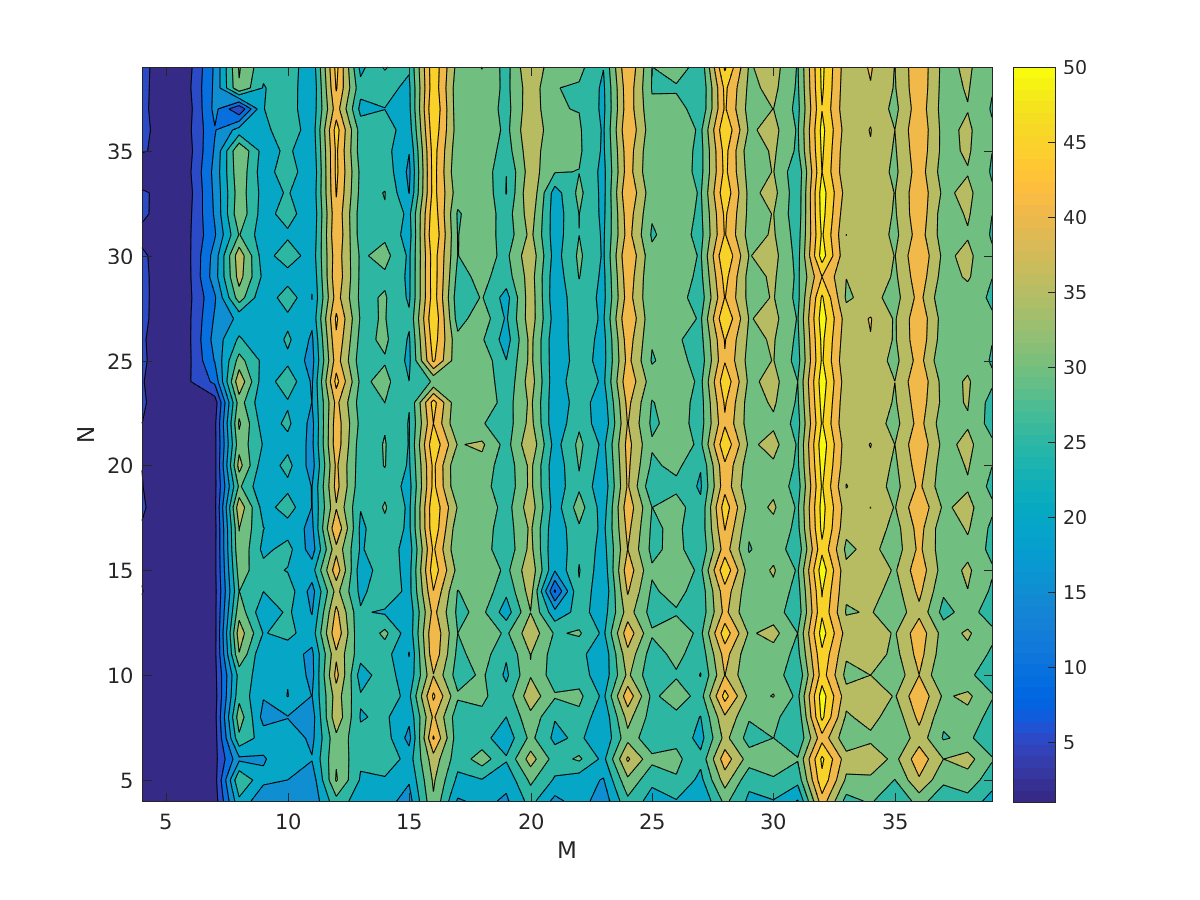
\includegraphics[width=\textwidth]{figures/contourSquareLeft}
\end{minipage}
\begin{minipage}{.48\textwidth}
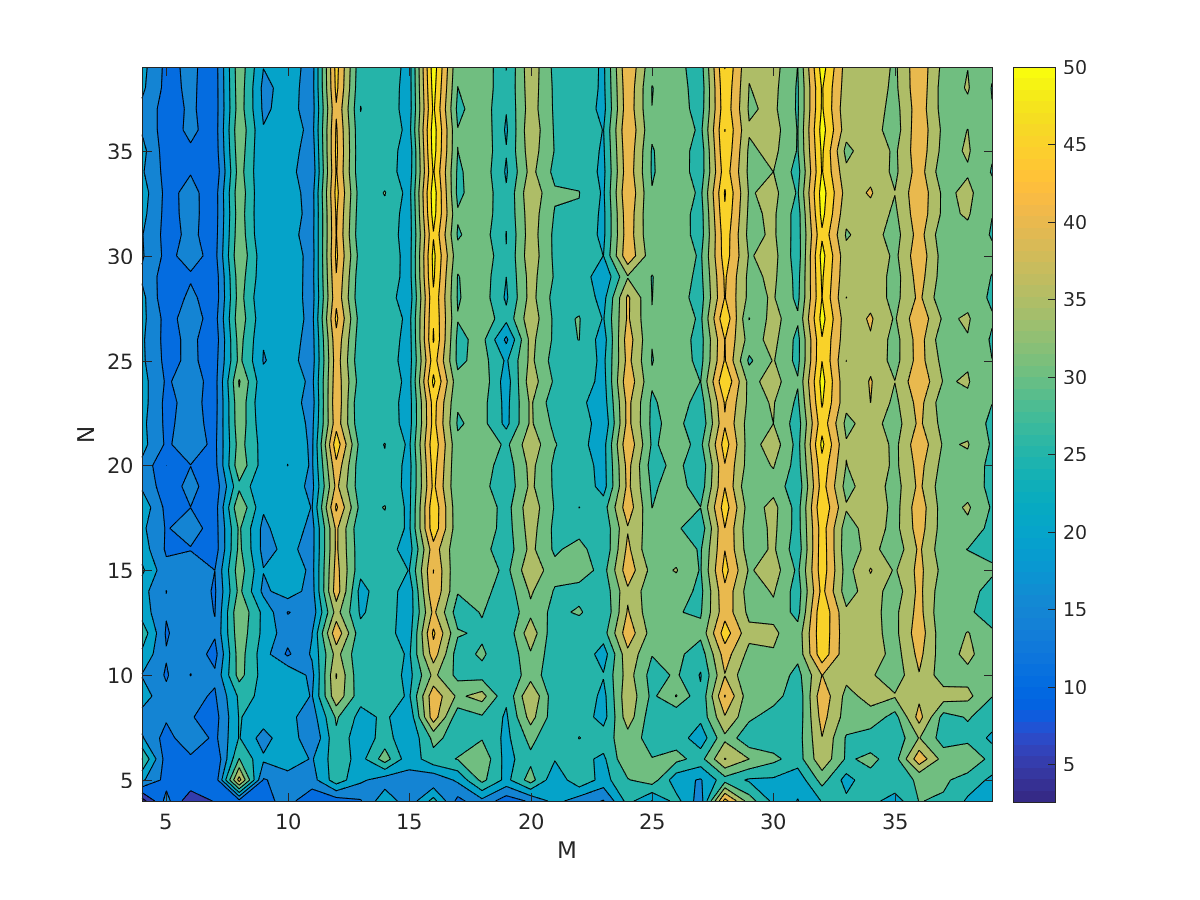
\includegraphics[width=\textwidth]{figures/contourSquareRight}
\end{minipage}
\caption{Performance of the dense matrix-matrix multiply in GFlops/s of $(M \times M) (M \times N)$ matrices (left) and $(M \times N) (N \times N)$ matrices (right).}\label{fig:contour}
\end{figure*}
Figure~\ref{fig:contour} lists the results for an average of ten runs on an Intel Xeon E3-1235v3 (``Haswell''). From a performance perspective the conclusions are as follows.
\begin{enumerate}
\item For very small-sized structures, the performance is poor in any case.
\item The system matrices should be padded in order to avoid performance valleys.
\item The plateaus are at $M=28$ and $M=32$ even if $N$ attains small values. The size of the square matrix takes a back seat to the structure of the tensor slice.
\end{enumerate}
The size of the system matrix is fixed and prescribed by the user. Typical dimensions are $4\times 4$ up to $10 \times 10$. The only opportunity for optimisation is padding, which has already been introduced. The second matrix, i.e. the tensor slice, behaves differently. One dimension of the tensor slice is fixed, of course. The other one, however, is not. This offers an opportunity for tuning. Looking at the figures, the key question is: How can the tensor slice be enlarged to hit a plateau? Section~\ref{sec:matricisation} takes up on this topic and discusses ideas on how this can be integrated into the code generator.

\subsection{Matricisation}\label{sec:matricisation}
From a performance perspective, it is better to compute one matrix-matrix multiply with one tall and thin tensor slice rather than a sequence of matrix-matrix multiplies with all small-sized matrices. Matricisation offers a means to jointly compute multiple matrix-matrix multiply, see Figure~\ref{fig:3}.  
\begin{figure}
\centering
\begin{subfigure}[b]{0.2\textwidth}
\centering
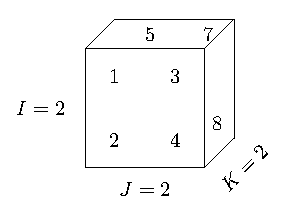
\includegraphics[scale=.6]{figures/figure4.eps}
\caption{Three-way tensor.}
\end{subfigure}
\begin{subfigure}[b]{0.2\textwidth}
\centering
\begin{tabular}{|cccc|}
\hline
1 & 3 & 5 & 7 \\
2 & 4 & 6 & 8 \\ \hline
\end{tabular}\vspace{1cm}
\caption{Matrix interpretation.}
\end{subfigure}
\caption{Storing frontal slices in column-major order.}\label{fig:4}
\end{figure}
The tensor slices, however, are scaled with the Gauss-Legendre quadrature weights. In fact it is the product of quadrature weights that impedes matricisation in a straightforward manner because of the dependence of the weights on the tensors slices. 


\begin{figure}[h!]
\centering
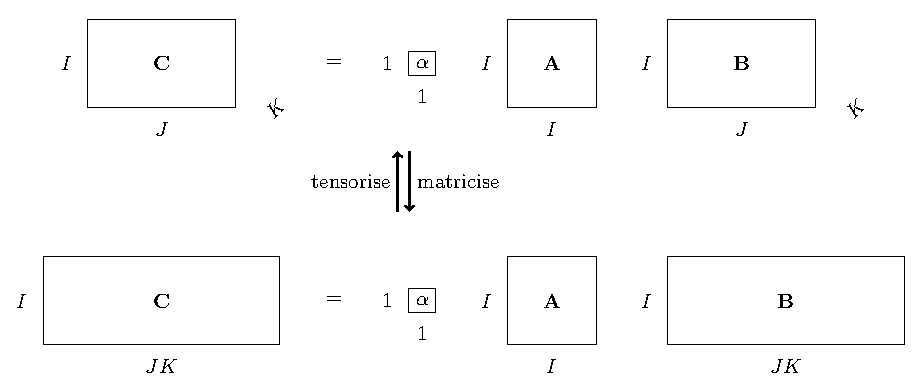
\includegraphics[width=.5\textwidth]{figures/figure3.eps}
\caption{Interpretation of the matrix-tensor product as GEMM.}\label{fig:3}
\end{figure}

There are three main ideas to nevertheless realise matricisation in ExaHyPE.
\begin{enumerate}
\item \textbf{Splitting.} Data structures such as the flux tensors hold dimension-dependent data. The flux tensor can therefore be split into smaller tensors for each direction, which in turn reordered in an advantageous way. The code generator already implements this idea.
\begin{figure*}
\begin{minipage}[t]{0.45\linewidth}
\begin{lstlisting}[language=fortran]
! x - direction 
DO j = 1, nDOF(2) 
 a = weight(j)/dx
 C(:,:,j) = C(:,:,j) + 
   a * MATMUL(Kxi, F(:,1,:,j))
ENDDO
! y - direction
DO i = 1, nDOF(1) 
 a = weight(i)/dx
 C(:,i,:) = C(:,i,:) + 
   a * MATMUL(Kxi, F(:,2,i,:))
ENDDO
\end{lstlisting}
\end{minipage}%
\hfill\vrule\hfill
\begin{minipage}[t]{0.45\linewidth}
\begin{lstlisting}[language=fortran]
! x - direction 
DO j = 1, nDOF(2) 
 a = weight(j)/dx
 C(:,:,j) = C(:,:,j) + 
   a * MATMUL(Kxi, Fx(:,:,j))
ENDDO
! y - direction
DO i = 1, nDOF(1) 
 a = weight(i)/dx
 C(:,i,:) = C(:,i,:) + 
   a * MATMUL(Kxi, Fy(:,:,i))
ENDDO
\end{lstlisting}
\end{minipage}
\caption{The generic code base (left) exhibits strided accesses to $\mathbf{F}$. Splitting $\mathbf{F}$ into $\mathbf{Fx}$, $\mathbf{Fy}$ and reordering $\mathbf{Fy}$ yields uniform access patterns enabling matricisation for both $x$- and $y$-direction (right).}\label{fig:code}
\end{figure*}

Recall that the way the tensors are accessed depends on the space direction. Wherever applicable, the tensors are therefore rearranged or reshaped to match the frontal variant of matricisation, illustrated in Figure~\ref{fig:3}. This holds for the flux tensors present in the space-time predictor and the volume integral. Figure~\ref{fig:code} gives the basic idea. Splitting up tensors into smaller tensors $\mathbf{Fx}$, $\mathbf{Fy}$ enables direction-dependent reordering of the tensor variables. The drawback, however, is that already small structures become even smaller. In terms of performance, it would be advantageous to group multiple operation of this type.
\item \textbf{Batched BLAS.} Multiple operations of the same kind can be glued together. Instead of a sequence of calls with different start addresses, the tensor slices should be considered as one joint operation. One idea of consolidating the quadrature weights and the matricisation idea is mimicking batched BLAS \cite{dongarra2016proposed}. Note that this idea takes place within a single element.

\item \textbf{Patches.} Reintroducing patches gives the opportunity to perform operations across multiple elements. The introduction of patches is not planned for the time being. Libxsmm does not offer an interface to incorporate arbitrary scalars into the matrix-matrix multiply. The workaround is the scaling of the system matrix before the gemm call. As multiple elements of the same spatial dimensions requires the same scaled system matrix, these operations could be glued together.
\end{enumerate}


%In other words, how can the tensor slice be artificially enlarged to chosen to be sufficiently It is inevitable to jointly compute multiple matrices. 
\section{Conclusion and Outlook}
The first version of the code generator is simplistic and mostly mimics the matrix-matrix multiplies of the generic code base. The driver files enable the usage of libxsmm as an assembly code generation back end. First optimisation steps include the padding of system matrices, the padding of tensors, and dimension-dependent splitting and reordering of tensor data. A pending step is the reintegration of the generated files into the Peano framework.

In terms of performance the quadrature weights pose a challenge. The current workaround of first scaling the system matrix with a quadrature weight and then calling the libxsmm-generated gemm implementation cannot be consolidated with the matricisation idea. The next steps will therefore address the integration of the quadrature weights. 

\bibliographystyle{abbrv}
\bibliography{report}

%\balancecolumns

\newpage
\appendix
\section{Performance measurements} \label{App:Performance measurements}

\subsection{Volume Kernel with 5, 9, 23 and 56 quantities (Haswell)} \label{sec:app1}

Figures \ref{fig:resultsVolumeHSW5}, \ref{fig:resultsVolumeHSW9}, \ref{fig:resultsVolumeHSW23} and \ref{fig:resultsVolumeHSW56}.

\begin{figure}[!h]
\begin{filecontents}{resultsVolumeHSW5.dat}
3,3.17,1.24,3.99
4,6.62,3.54,9.7
5,12.86,6.47,19.25
6,21.56,11.22,34.63
7,35.27,17.53,57.93
8,54.06,32.32,91.47
\end{filecontents}
\begin{tikzpicture}
\begin{axis}[xlabel={order},ylabel={Runtime in $\mu$s},legend style={at={(0,1)},anchor=north west}, legend cell align=left]
% Graph column 2 versus column 0
\addplot[color=black,mark=square*] table[x index=0,y index=3,col sep=comma] {resultsVolumeHSW5.dat};
\addlegendentry{Generic C++} % column right
% Graph column 3 versus column 0
\addplot[color=red,mark=otimes*] table[x index=0,y index=1,col sep=comma] {resultsVolumeHSW5.dat};
\addlegendentry{Generic Fortran} % column left
% Graph column 1 versus column 0    
\addplot[color=blue,mark=triangle*] table[x index=0,y index=2,col sep=comma] {resultsVolumeHSW5.dat};
\addlegendentry{Optimised} % column middle
\end{axis}
\end{tikzpicture}
\caption{Haswell (nVar=5) - Performance comparison of the generic and optimised version of the volume kernel.}\label{fig:resultsVolumeHSW5}
\end{figure}

\begin{figure}[!h]
\begin{filecontents}{resultsVolumeHSW9.dat}
3,6.516,1.49589,6.98237
4,13.804,4.53058,15.9852
5,25.885,8.08679,32.0277
6,43.346,12.9495,58.4853
7,68.516,21.2638,97.9753
8,106.25,38.0867,157.696
\end{filecontents}
\begin{tikzpicture}
\begin{axis}[xlabel={order},ylabel={Runtime in $\mu$s},legend style={at={(0,1)},anchor=north west}, legend cell align=left]
% Graph column 2 versus column 0
\addplot[color=black,mark=square*] table[x index=0,y index=3,col sep=comma] {resultsVolumeHSW9.dat};
\addlegendentry{Generic C++} % column right
% Graph column 3 versus column 0
\addplot[color=red,mark=otimes*] table[x index=0,y index=1,col sep=comma] {resultsVolumeHSW9.dat};
\addlegendentry{Generic Fortran} % column left
% Graph column 1 versus column 0    
\addplot[color=blue,mark=triangle*] table[x index=0,y index=2,col sep=comma] {resultsVolumeHSW9.dat};
\addlegendentry{Optimised} % column middle
\end{axis}
\end{tikzpicture}
\caption{Haswell (nVar=9) - Performance comparison of the generic and optimised version of the volume kernel.}\label{fig:resultsVolumeHSW9}
\end{figure}

\begin{figure}[!h]
\begin{filecontents}{resultsVolumeHSW23.dat}
3,11.988,2.94588,17.6063
4,25.477,10.0396,43.1139
5,47.530,16.6924,86.9704
6,80.669,24.2394,159.446
7,128.74,40.5277,266.781
8,194.34,67.1205,422.983
\end{filecontents}
\begin{tikzpicture}
\begin{axis}[xlabel={order},ylabel={Runtime in $\mu$s},legend style={at={(0,1)},anchor=north west}, legend cell align=left]
% Graph column 2 versus column 0
\addplot[color=black,mark=square*] table[x index=0,y index=3,col sep=comma] {resultsVolumeHSW23.dat};
\addlegendentry{Generic C++} % column right
% Graph column 3 versus column 0
\addplot[color=red,mark=otimes*] table[x index=0,y index=1,col sep=comma] {resultsVolumeHSW23.dat};
\addlegendentry{Generic Fortran} % column left
% Graph column 1 versus column 0    
\addplot[color=blue,mark=triangle*] table[x index=0,y index=2,col sep=comma] {resultsVolumeHSW23.dat};
\addlegendentry{Optimised} % column middle
\end{axis}
\end{tikzpicture}
\caption{Haswell (nVar=23) - Performance comparison of the generic and optimised version of the volume kernel.}\label{fig:resultsVolumeHSW23}
\end{figure}

\begin{figure}[!h]
\begin{filecontents}{resultsVolumeHSW56.dat}
3,23.609,5.1009,42.9111
4,49.951,16.1373,101.721
5,95.661,26.1655,207.249
6,162.52,45.2881,378.194
7,255.21,72.1924,637.574
8,382.19,116.017,1011.62
\end{filecontents}
\begin{tikzpicture}
\begin{axis}[xlabel={order},ylabel={Runtime in $\mu$s},legend style={at={(0,1)},anchor=north west}, legend cell align=left]
% Graph column 2 versus column 0
\addplot[color=black,mark=square*] table[x index=0,y index=3,col sep=comma] {resultsVolumeHSW56.dat};
\addlegendentry{Generic C++} % column right
% Graph column 3 versus column 0
\addplot[color=red,mark=otimes*] table[x index=0,y index=1,col sep=comma] {resultsVolumeHSW56.dat};
\addlegendentry{Generic Fortran} % column left
% Graph column 1 versus column 0    
\addplot[color=blue,mark=triangle*] table[x index=0,y index=2,col sep=comma] {resultsVolumeHSW56.dat};
\addlegendentry{Optimised} % column middle
\end{axis}
\end{tikzpicture}
\caption{Haswell (nVar=56) - Performance comparison of the generic and optimised version of the volume kernel.}\label{fig:resultsVolumeHSW56}
\end{figure}

\subsection{KNL measurements for 9 quantities} \label{sec:app2}

Figures \ref{fig:resultsPicardKNL9}, \ref{fig:resultsVolumeKNL9} and \ref{fig:resultsPredictorKNL9}

\begin{figure}[!h]
\begin{filecontents}{resultsPicardKNL9.dat}
% order fortran  optimised   generic
3,478.40,113.836,2266.43
4,1184.2,600.758,7051
5,4942.0,1492.23,17843.8
6,9540.6,4481.87,39529.4
7,28543.7,9043.53,79266.7
8,55851,19236.1,167598
% fluctuates heavily.
\end{filecontents}
\pgfplotsset{scaled y ticks=false}
\begin{tikzpicture}
\begin{axis}[xlabel={order},ylabel={Runtime in $\mu$s},legend style={at={(0,1)},anchor=north west}, legend cell align=left]
% Graph column 1 versus column 0
\addplot[color=red,mark=otimes*] table[x index=0,y index=1,col sep=comma] {resultsPicardKNL9.dat};
\addlegendentry{Generic Fortran} % columns left
% Graph column 2 versus column 0
\addplot[color=blue,mark=triangle*] table[x index=0,y index=2,col sep=comma] {resultsPicardKNL9.dat};
\addlegendentry{Optimised} % column middle
% Graph column 3 versus column 0
\addplot[color=black,mark=square*] table[x index=0,y index=3,col sep=comma] {resultsPicardKNL9.dat};
\addlegendentry{Generic C++} % column right
\end{axis}
\end{tikzpicture}
\caption{KNL (nVar=9) - Performance comparison of various implementations of the Picard loop without the evaluation of the 3D Euler flux function.}\label{fig:resultsPicardKNL9}
\end{figure}


\begin{figure}[!h]
\begin{filecontents}{resultsVolumeKNL9.dat}
3,13.441,8.38603,57.3444
4,29.613,17.5064,125.507
5,58.634,28.84,240.093
6,100.93,55.8389,415.067
7,235.84,069.9527,689.63
8,418.90,123.351,1078.78
\end{filecontents}
\begin{tikzpicture}
\begin{axis}[xlabel={order},ylabel={Runtime in $\mu$s},legend style={at={(0,1)},anchor=north west}, legend cell align=left]
% Graph column 2 versus column 0
\addplot[color=black,mark=square*] table[x index=0,y index=3,col sep=comma] {resultsVolumeKNL9.dat};
\addlegendentry{Generic C++} % column right
% Graph column 3 versus column 0
\addplot[color=red,mark=otimes*] table[x index=0,y index=1,col sep=comma] {resultsVolumeKNL9.dat};
\addlegendentry{Generic Fortran} % column left
% Graph column 1 versus column 0    
\addplot[color=blue,mark=triangle*] table[x index=0,y index=2,col sep=comma] {resultsVolumeKNL9.dat};
\addlegendentry{Optimised (generated)} % column middle
\end{axis}
\end{tikzpicture}
\caption{KNL (nVar=9) - Performance comparison of the generic and optimised version of the volume kernel.}\label{fig:resultsVolumeKNL9}
\end{figure}

\begin{figure}[!h]
\begin{filecontents}{resultsPredictorKNL9.dat}
3,26.683,10.1179,41.3169
4,70.792,22.1205,76.2355
5,139.83,67.6069,228.711
6,248.93,200.171,432.406
7,414.31,338.915,586.784
8,859.87,499.727,1102.92
\end{filecontents} 
\begin{tikzpicture}
\begin{axis}[xlabel={order},ylabel={Runtime in $\mu$s},legend style={at={(0,1)},anchor=north west}, legend cell align=left]
% Graph column 2 versus column 0
\addplot[color=black,mark=square*] table[x index=0,y index=3,col sep=comma] {resultsPredictorKNL9.dat};
\addlegendentry{Generic C++} % column right
% Graph column 3 versus column 0
\addplot[color=red,mark=otimes*] table[x index=0,y index=1,col sep=comma] {resultsPredictorKNL9.dat};
\addlegendentry{Generic Fortran} % column left
% Graph column 1 versus column 0    
\addplot[color=blue,mark=triangle*] table[x index=0,y index=2,col sep=comma] {resultsPredictorKNL9.dat};
\addlegendentry{Optimised} % column middle
\end{axis}
\end{tikzpicture}
\caption{KNL (nVar=9) - Performance comparison of the generic and optimised version of the time averaging.}\label{fig:resultsPredictorKNL9}
\end{figure}

\end{document}
